\section{eBPF}\label{sec:ebpf_bg}
In 1992 a technology called `Berkeley Packet Filter' (BPF) was introduced into 
the Unix kernel.
By using BPF it is possible to attach a small BPF-program to some pre-defined hook points in 
the network stack of the kernel and filter packets there in a stateless manner.
This provided more efficiency since the packets did not need to be copied into 
userspace anymore but could directly be processed in the kernel.
A need for better tracing capabilities of the Linux kernel led to the development 
of an extended version of BPF called ``eBPF'' which was introduced in 2014 and 
heavily influenced by a tracing tool called ``dtrace''~\parencite{ebpf-intro-tigera}.

\subsection{eBPF Hook Points}
The Linux kernel offers several hook points where eBPF-programs can be attached to.
There are two prominent ones that we considered for our suggested setup.
The first one allows one to access the Traffic Control (TC) subsystem
while the second one allows one to access the eXpress Data Path (XDP) subsystem.

XDP would generally provide a better performance since it is located 
lower on the network stack, namely directly in the NIC driver, than the 
TC-hook point, which is located in the link-layer.
TC on the other hand offers a more versatile way of packet processing since 
the used \verb|sk_buff| provides access to metadata that is not available when using 
XDP and its \verb|xdp_buff|.
% https://liuhangbin.netlify.app/post/ebpf-and-xdp/ % TODO: is this citable?
What ultimately led us to choose TC over XDP was however the fact that 
XDP only allows ingress packet processing while TC allows for both ingress and egress.
That means that with XDP we would not have been able to redirect packets to be handled 
at egress which is crucial for the fast-relay setup we are aiming for.

% The XDP hook, which is directly located in the NIC-driver, lies lower in the network 
% stack than the TC-hook, which is located in the link-layer.
% Despite being higher up in the network stack, the TC-hook has the big advantage that
% it offers ingress and egress processing while the XDP-hook is available for ingress 
% processing only.
% This makes the XDP-hook suboptimal for the implementation of fast-relays since 
% they heavily rely on processing packets at egress, after those were redirected
% from ingress.
Figure~\autoref{fig:ebpf-hooks} illustrates again the relative positions of the TC and
XDP hook points in the network stack.

\begin{figure}[htbp]
    \centering
    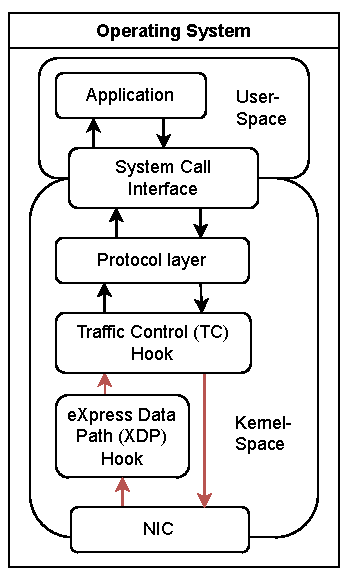
\includegraphics[width=0.3\textwidth]{figures/02_background/hook-point-locations.drawio.pdf}
    \caption{Abstracted view of Traffic Control (TC) and eXpress Data Path (XDP) hook points
    in the Linux kernel network stack.
    The red loop indicates the `short-cut' that is utilized by the fast-relay.
    TC hook allows redirection directly to egress while XDP hook is only available
    for ingress processing.
    }\label{fig:ebpf-hooks}
\end{figure}

\subsection{Traffic Control Queuing Disciplines}
The Linux Traffic Control Subsystem uses Queuing Disciplines (qdiscs) to define how packets
are handled. TODO

\subsection{eBPF Verifier}
Since eBPF programs are executed in the kernel it is quite obvious that extensive
security checks need to be in place to ensure that the kernel does not experience 
problems like infinite loops, accesses to invalid memory locations or other security 
related issues.
This explains the existence of the so-called `BPF-verifier' which inspects 
every BPF-program for its safety by simulating possible program paths, 
looking at the graph representation of the program and more~\parencite{ebpf-verifier}.
This imposes some restrictions on the complexity of the programs that can be 
used within the kernel.
In our case this did not impose too many issues though since we do not rely on 
very complex control structures.

\subsection{Important eBPF Concepts}
One of the most important concepts in eBPF which we do however use quite extensively is 
the `eBPF-map'.
Such a map boils down to a section in memory that is reserved for the eBPF-program
and which can be used as a key-value store for arbitrary data.
This part of memory can then also be accessed from userspace and thus provides the main 
way of communication between the eBPF-program and our application.
When we define an eBPF-map we can choose between different types as well as configure
size, key-type, value-type and the way the map is stored. % TODO: surely there is more one can define
An example of two eBPF-map definitions can be seen in~\autoref{lst:ebpf-map}.
It shows two different types of maps, a hash map and a ring buffer, that are used in
our fast-relay setup.
Some relevant map types are listed in table~\autoref{tab:ebpf-map-types}.


\begin{figure}[htbp]
    \begin{lstlisting}[style=CStyle]
        struct {
            __uint(type, BPF_MAP_TYPE_HASH);        // Hash map
            __type(key, struct client_info_key_t);  // Specific client key
            __type(value, uint32_t);                // 32 bit id
            __uint(max_entries, MAX_CLIENTS);       // Maximum number of clients
            __uint(pinning, LIBBPF_PIN_BY_NAME);    // Pin by name to the tc filesystem
        } client_id SEC(".maps");

        struct {
            __uint(type, BPF_MAP_TYPE_RINGBUF);     // Ring buffer
            __uint(max_entries, MAX_PACKET_EVENTS); // Maximum number of packet events
            __uint(pinning, LIBBPF_PIN_BY_NAME);    // Pin by name to the tc filesystem
        } packet_events SEC(".maps");
    \end{lstlisting}
    \caption{Examplary eBPF map definitions.}\label{lst:ebpf-map}
\end{figure}

\FloatBarrier

\begin{table}[htbp]
    \centering
    \begin{tabular}{L{7cm}L{7cm}}
        \toprule
            Type & Description \\
        \midrule
            BPF\_MAP\_TYPE\_HASH & A hash map where keys and values can be arbitrarily defined. \\
        \midrule
            BPF\_MAP\_TYPE\_PERCPU\_HASH & A hash map with separate values for each CPU, providing improved performance in multi-core environments. \\
        \midrule
            BPF\_MAP\_TYPE\_ARRAY & An array map that allows random access to elements by index. \\
        \midrule
            BPF\_MAP\_TYPE\_PERCPU\_ARRAY & An array map with separate values for each CPU, useful for per-CPU data storage. \\
        \midrule
            BPF\_MAP\_TYPE\_RINGBUF & A ring buffer for implementing high-performance data queues. \\
        \bottomrule
    \end{tabular}
    \caption[TODO: add this to tables and figures for better naming]{Some eBPF map types. (defined in /usr/include/linux/bpf.h)}\label{tab:eBPF-map-types}
\end{table}

\subsection{eBPF and Fast-Relays}
TODO

\FloatBarrier

\begin{figure}[htbp] % TODO: where to put this?
    \centering
    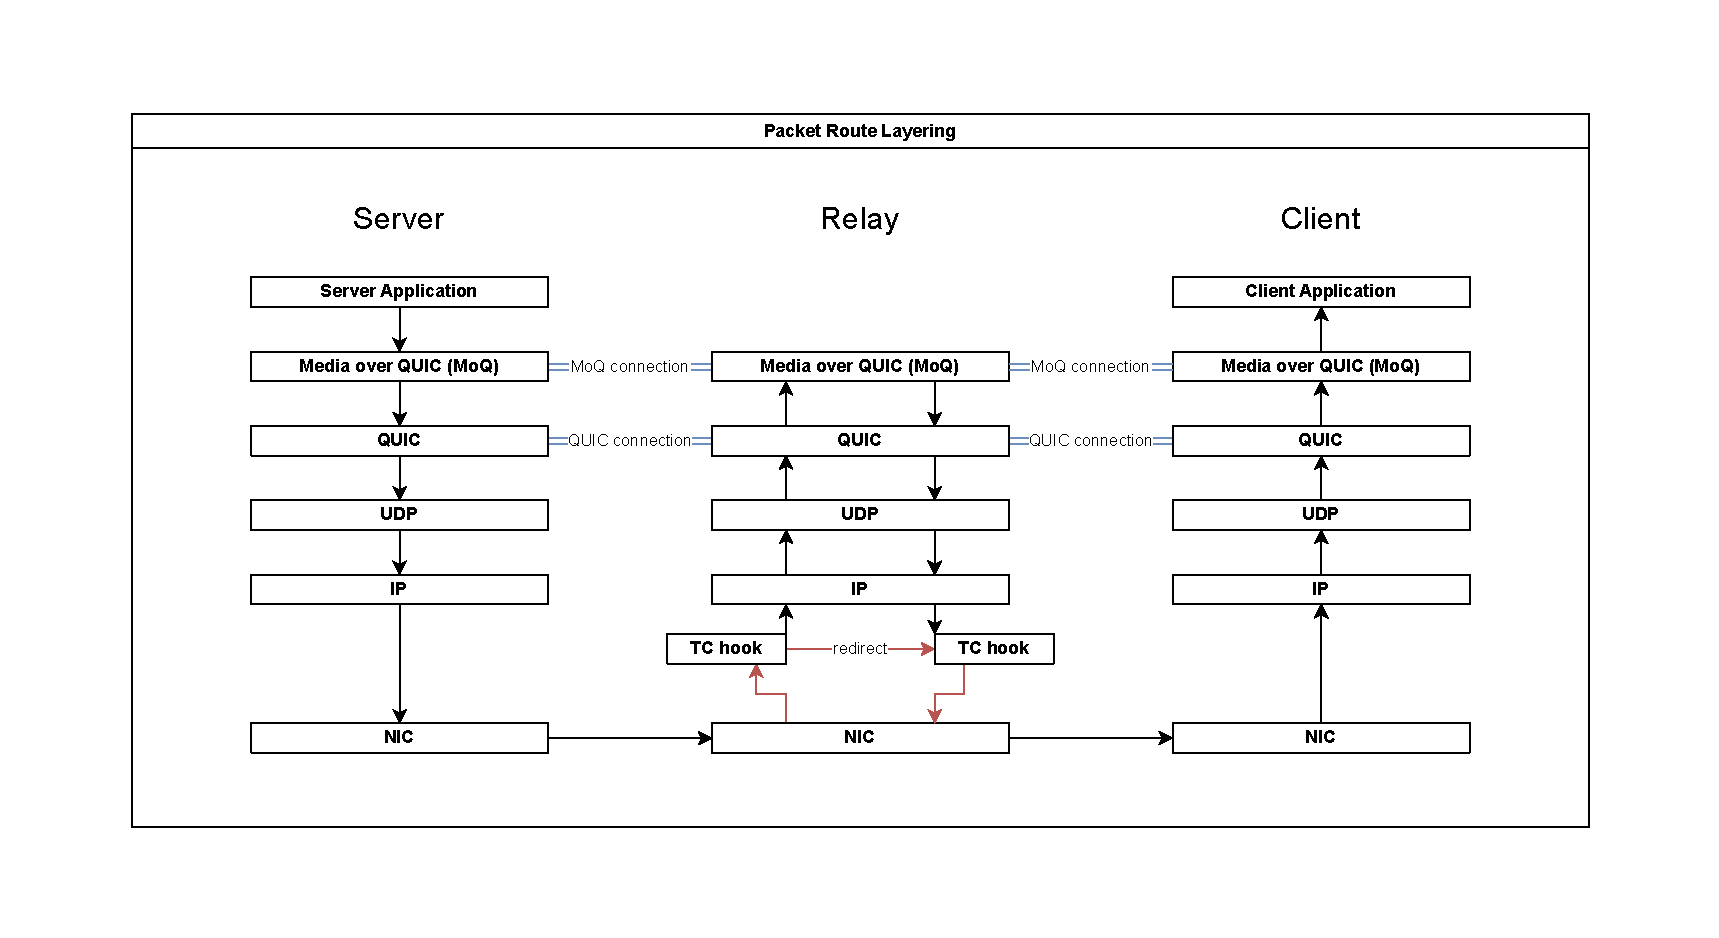
\includegraphics[width=\textwidth]{figures/02_background/route-layering.drawio.pdf}
    \caption{Conventional layers of a network stack for client, server and relay.
    The red loop indicates again the `short-cut' that is utilized by the fast-relay and 
    based on eBPF packet-forwarding.
    This avoids the need for the packet to traverse the entire network stack of the relay 
    up to the userspace.}\label{fig:route-layering}
\end{figure}
